\documentclass[11pt]{article}
\usepackage{graphicx}
\usepackage{hyperref}
\usepackage{natbib}

\setlength{\textwidth}{6.5in}
\setlength{\headheight}{0in}
\setlength{\textheight}{8.0in}
\setlength{\hoffset}{0in}
\setlength{\voffset}{0in}
\setlength{\oddsidemargin}{0in}
\setlength{\evensidemargin}{0in}

\title{Computational Physics: Problem Set 9}

\author{Zifeng Li}
\begin{document}
\maketitle

\section{Questions}

\subsection{Question 1}

Using the given constants, we can calculate the matrix and from that we can get
the vector for solving the linear system. The resulted wave function should be
an array with N complex numbers.

The first five elements are: [ 4.08093184e-278-3.10068560e-278j -2.59781065e-278-2.03625934e-277j
 -7.99366914e-277-2.86098508e-277j -2.56554479e-276+2.40530824e-276j
  4.01492601e-276+1.39993998e-275j].

Using the Crank-Nicolson method, we can plot the real part of the wavefunction at
each of these time steps. The graph below is the result.
\begin{figure}[b!]
\centering
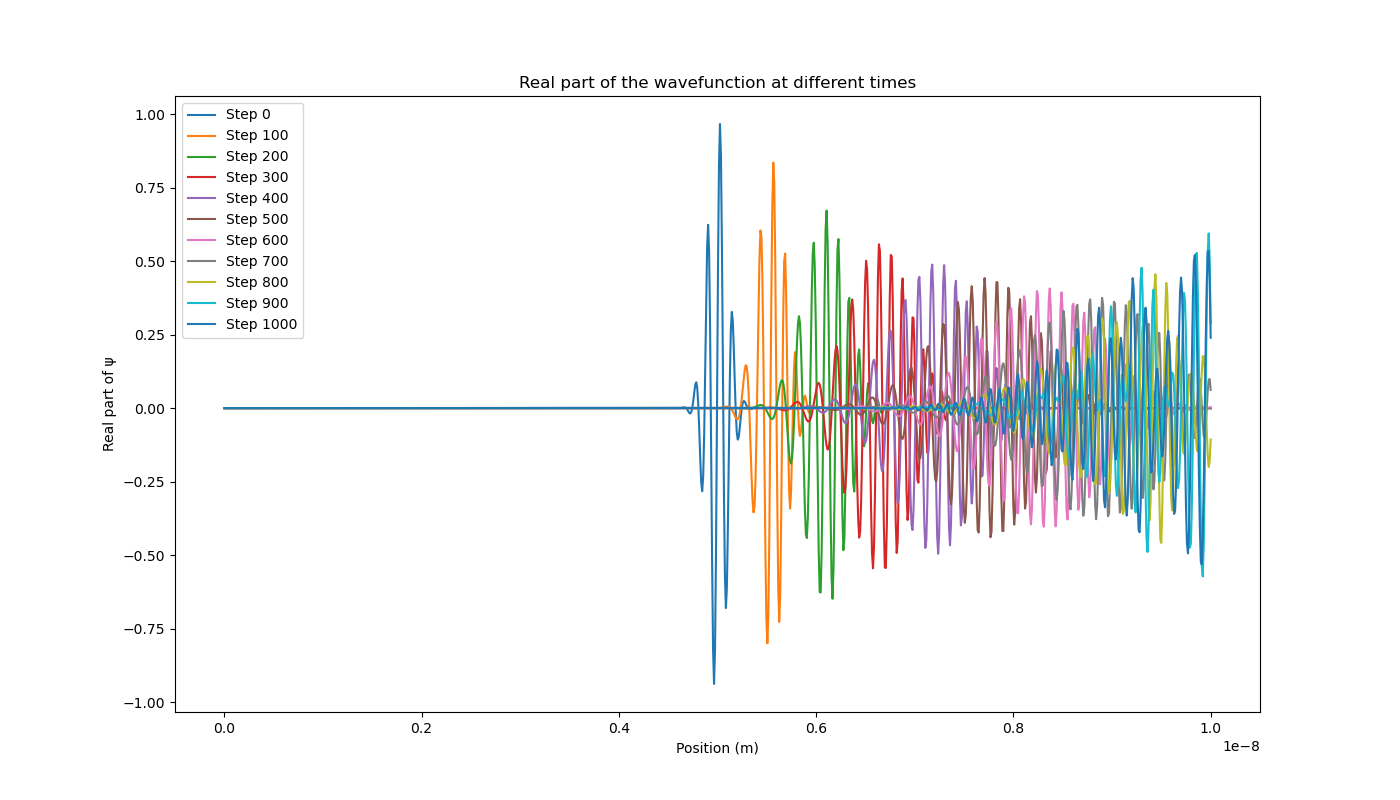
\includegraphics[width=0.95\textwidth]{Real part of the wavefunction at different times.png}
\end{figure}




\end{document}
